% A LaTeX (non-official) template for ISAE projects reports
% Copyright (C) 2014 Damien Roque
% Version: 0.2
% Author: Damien Roque <damien.roque_AT_isae.fr>

\documentclass[a4paper,12pt,oneside]{book}
\usepackage[utf8]{inputenc}
\usepackage[T1]{fontenc}
\usepackage[english]{babel} % If you write in English
\usepackage{a4wide}
\usepackage{graphicx}
\graphicspath{{images/}}
\usepackage{subfig}
\usepackage{tikz}
\usetikzlibrary{shapes,arrows}
\usepackage{pgfplots}
\pgfplotsset{compat=newest}
\pgfplotsset{plot coordinates/math parser=false}
\newlength\figureheight
\newlength\figurewidth
\pgfkeys{/pgf/number format/.cd,
set decimal separator={,\!},
1000 sep={\,},
}
\usepackage{ifthen}
\usepackage{ifpdf}
\usepackage{enumitem}
\ifpdf
\usepackage[pdftex]{hyperref}
\else
\usepackage{hyperref}
\fi
\usepackage{color}
\hypersetup{%
colorlinks=true,
linkcolor=black,
citecolor=black,
urlcolor=black}

\renewcommand{\baselinestretch}{1.05}
\usepackage{fancyhdr}
\pagestyle{fancy}
\fancyfoot{}
\fancyhead[LE,RO]{\bfseries\thepage}
\fancyhead[RE]{\bfseries\nouppercase{\leftmark}}
\fancyhead[LO]{\bfseries\nouppercase{\rightmark}}
\setlength{\headheight}{15pt}

\let\headruleORIG\headrule
\renewcommand{\headrule}{\color{black} \headruleORIG}
\renewcommand{\headrulewidth}{1.0pt}
\usepackage{colortbl}
\arrayrulecolor{black}

\fancypagestyle{plain}{
  \fancyhead{}
  \fancyfoot[C]{\thepage}
  \renewcommand{\headrulewidth}{0pt}
}

\makeatletter
\def\@textbottom{\vskip \z@ \@plus 1pt}
\let\@texttop\relax
\makeatother

\makeatletter
\def\cleardoublepage{\clearpage\if@twoside \ifodd\c@page\else%
  \hbox{}%
  \thispagestyle{empty}%
  \newpage%
  \if@twocolumn\hbox{}\newpage\fi\fi\fi}
\makeatother

\usepackage{amsthm}
\usepackage{amssymb,amsmath,bbm}
\usepackage{array}
\usepackage{bm}
\usepackage{multirow}
\usepackage[footnote]{acronym}


\usepackage[figuresleft]{rotating}

\newcommand*{\SET}[1]  {\ensuremath{\mathbf{#1}}}
\newcommand*{\VEC}[1]  {\ensuremath{\boldsymbol{#1}}}
\newcommand*{\FAM}[1]  {\ensuremath{\boldsymbol{#1}}}
\newcommand*{\MAT}[1]  {\ensuremath{\boldsymbol{#1}}}
\newcommand*{\OP}[1]  {\ensuremath{\mathrm{#1}}}
\newcommand*{\NORM}[1]  {\ensuremath{\left\|#1\right\|}}
\newcommand*{\DPR}[2]  {\ensuremath{\left \langle #1,#2 \right \rangle}}
\newcommand*{\calbf}[1]  {\ensuremath{\boldsymbol{\mathcal{#1}}}}
\newcommand*{\shift}[1]  {\ensuremath{\boldsymbol{#1}}}

\newcommand{\eqdef}{\stackrel{\mathrm{def}}{=}}
\newcommand{\argmax}{\operatornamewithlimits{argmax}}
\newcommand{\argmin}{\operatornamewithlimits{argmin}}
\newcommand{\ud}{\, \mathrm{d}}
\newcommand{\vect}{\text{Vect}}
\newcommand{\sinc}{\ensuremath{\mathrm{sinc}}}
\newcommand{\esp}{\ensuremath{\mathbb{E}}}
\newcommand{\hilbert}{\ensuremath{\mathcal{H}}}
\newcommand{\fourier}{\ensuremath{\mathcal{F}}}
\newcommand{\sgn}{\text{sgn}}
\newcommand{\intTT}{\int_{-T}^{T}}
\newcommand{\intT}{\int_{-\frac{T}{2}}^{\frac{T}{2}}}
\newcommand{\intinf}{\int_{-\infty}^{+\infty}}
\newcommand{\Sh}{\ensuremath{\boldsymbol{S}}}
\newcommand{\C}{\SET{C}}
\newcommand{\R}{\SET{R}}
\newcommand{\Z}{\SET{Z}}
\newcommand{\N}{\SET{N}}
\newcommand{\K}{\SET{K}}
\newcommand{\reel}{\mathcal{R}}
\newcommand{\imag}{\mathcal{I}}
\newcommand{\cmnr}{c_{m,n}^\reel}
\newcommand{\cmni}{c_{m,n}^\imag}
\newcommand{\cnr}{c_{n}^\reel}
\newcommand{\cni}{c_{n}^\imag}
\newcommand{\tproto}{g}
\newcommand{\rproto}{\check{g}}
\newcommand{\LR}{\mathcal{L}_2(\SET{R})}
\newcommand{\LZ}{\ell_2(\SET{Z})}
\newcommand{\LZI}[1]{\ell_2(\SET{#1})}
\newcommand{\LZZ}{\ell_2(\SET{Z}^2)}
\newcommand{\diag}{\operatorname{diag}}
\newcommand{\noise}{z}
\newcommand{\Noise}{Z}
\newcommand{\filtnoise}{\zeta}
\newcommand{\tp}{g}
\newcommand{\rp}{\check{g}}
\newcommand{\TP}{G}
\newcommand{\RP}{\check{G}}
\newcommand{\dmin}{d_{\mathrm{min}}}
\newcommand{\Dmin}{D_{\mathrm{min}}}
\newcommand{\Image}{\ensuremath{\text{Im}}}
\newcommand{\Span}{\ensuremath{\text{Span}}}

\newtheoremstyle{break}
  {11pt}{11pt}%
  {\itshape}{}%
  {\bfseries}{}%
  {\newline}{}%
\theoremstyle{break}

%\theoremstyle{definition}
\newtheorem{definition}{Définition}[chapter]

%\theoremstyle{definition}
\newtheorem{theoreme}{Théorème}[chapter]

%\theoremstyle{remark}
\newtheorem{remarque}{Remarque}[chapter]

%\theoremstyle{plain}
\newtheorem{propriete}{Propriété}[chapter]
\newtheorem{exemple}{Exemple}[chapter]

\parskip=5pt
%\sloppy

\definecolor{RedBg}{rgb}{1,0.8,0.8}

\newcolumntype{r}{>{\columncolor{RedBg}}c}

\begin{document}

%%%%%%%%%%%%%%%%%%
%%% First page %%%
%%%%%%%%%%%%%%%%%%

\begin{titlepage}
\begin{center}

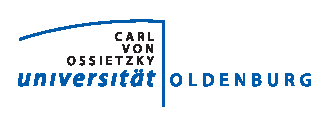
\includegraphics[width=0.6\textwidth]{uol}\\[1cm]

{\large Modellierungspraktikum}\\[0.5cm]

{\large SS 2019}\\[0.5cm]

% Title
\rule{\linewidth}{0.5mm} \\[0.4cm]
{ \huge \bfseries Cross Correlation of two Ohrnstein Uhlenbeck Processes with Delayed Noise \\[0.4cm] }
\rule{\linewidth}{0.5mm} \\[1.5cm]

% Author and supervisor
\noindent
\begin{minipage}{0.4\textwidth}
  \begin{flushleft} \large
    \emph{Author}\\
    Tjark Smalla\\
  \end{flushleft}
\end{minipage}%
\begin{minipage}{0.4\textwidth}
  \begin{flushright} \large
    \emph{Professor} \\
    PD. Jan Freund
  \end{flushright}
\end{minipage}

\vfill

% Bottom of the page
{\large \today}

\end{center}
\end{titlepage}

%%%%%%%%%%%%%%%%%%%%%%%%%%%%%
%%% Non-significant pages %%%
%%%%%%%%%%%%%%%%%%%%%%%%%%%%%

\frontmatter

\tableofcontents

\clearpage
\listoffigures

\clearpage
\chapter*{Acronyms}
\begin{acronym}[CP-OFDMX] % Give the longest acronym here
\acro{OU}{Ohrnstein Uhlenbeck}
\acro{CCF}{cross correlation function}
\acro{ACF}{auto correlation function}
\acro{SDE}{stochastic differential equation}
\acro{EM}{Euler-Maruyama Method}
\acro{FWAHH}{Full Width at Half Height}
\end{acronym}

%%%%%%%%%%%%%%%%%%%%%%%%%%%%%%%%%%%%%%%%%%%%
%%% Content of the report and references %%%
%%%%%%%%%%%%%%%%%%%%%%%%%%%%%%%%%%%%%%%%%%%%

\mainmatter
\pagestyle{fancy}

\cleardoublepage
\chapter{Introduction}\label{ch/intro}
Aim of this report is to study the \ac{CCF} properties of two connected \ac{OU} processes under changing parameterization.
Both processes are powered by gaussian noise, whereas the second process is powered by a linear combination of a time delayed version of the first noise and a second gaussian noise process. The two independent gaussian noise processes will be from now on referred to as noise 1 and noise 2. The noise resulting from the linear combination of noise 1 and noise 2 will be referred to as mixed noise. Noise 1 is powering \ac{OU} process 1 and the mixed noise powers \ac{OU} process 2. For better readability, the first process is from now on referred to as OU1 and the second process as OU2.
To further analyze the dependency of the \ac{CCF}s characteristics on the noise, the gaussian noise is replaced by a red noise.
The current chapter is supposed to define the model under study(\ref{s/model})) as well as which parameters will be analyzed(\ref{s/intro/parameter}).
Chapter \ref{ch/methodology} explains how the \ac{CCF} was estimated from an ensemble of \ac{OU} realizations. Section \ref{s/meth/num} explains in more detail which method was used to solve the \ac{SDE} defined in equation \ref{m/ou1n} and \ref{m/ou2n} while section \ref{s/meth/simulation} gives an overview over the simulation parameters and methods.
The resulting \ac{ACF}s and \ac{CCF}s are displayd in chapter \ref{ch/results}. A visualization of correlation effects caused by parameterization is provided in section \ref{s/r/correlation_sym}.
Finally chapter \ref{ch/conclusion} summarizes which conclusions can be drawn from the simulated results.

The reader might be interested in additional plots which can be found in chapter \ref{ch/appendix}.

\section{Model Definition}\label{s/model}
The \ac{OU} processes under study are given by following langevin equations

\begin{equation}\label{m/ou1}
	\dot{x_1}=-\frac{x_1}{\tau_1} + \sqrt{\frac{2\sigma^2}{\tau_1}}\xi_1(t)
\end{equation}

\begin{equation}\label{m/ou2}
	\dot{x_2}=-\frac{x_2}{\tau_2} + \sqrt{\frac{2\sigma^2}{\tau_2}}\times[\sqrt{\epsilon^2}\xi_1(t - T) + \sqrt{1-\epsilon^2} \xi_2(t)]
\end{equation}
with relaxation rate $\tau$, noise intensity $\sigma^2$ and coupling delay $T$.
Assuming a shared dimension of $x_1$ and $x_2$,  $\sigma$ can assumed to be 1 which leads to following normalized processes:

\begin{equation}\label{m/ou1n}
\dot{x_1}=-\frac{x_1}{\tau_1} + \sqrt{\frac{2}{\tau_1}}\xi_1(t)
\end{equation}

\begin{equation}\label{m/ou2n}
\dot{x_2}=-\frac{x_2}{\tau_2} + \sqrt{\frac{2}{\tau_2}}\times[\sqrt{\epsilon^2}\xi_1(t - 1) + \sqrt{1-\epsilon^2} \xi_2(t)].
\end{equation}

The impact of the noises \ac{ACF} properties is studied by assuming white and red spectral characteristics. Thus the \ac{ACF} of noise 1 and 2($\xi_1$, $\xi_2$) is given by

% TODO add comment for cases red and white nosie behin the condition
% TODO remake sentence before equation
\begin{equation}
	\langle x_i(t)x_j(s)\rangle = \delta_{i,j}
	\begin{cases} 
	\delta(t-s)  \quad \text{for white noise}\\
	e^{-\gamma_i |t-s|} \quad \text{for red noise}
	\end{cases}
\end{equation}

with $\gamma$ controlling the correlation time of the the red noise.

\section{Parameter Under Study}\label{s/intro/parameter}
Special attention is given to the effects resulting from changes in the parameters controlling the weighting of the linear combination $\epsilon$, the relaxation coefficient $\tau$ as well as the correlation time $\gamma$.

% TODO Expectation

% --------------------------------------------------------------------------------------------
\chapter{Methodology}\label{ch/methodology}
To analyze parameterization effects on the \ac{ACF}s and \ac{CCF}s, both are estimated from an ensemble of bivariate time series generated from the \ac{SDE} defined in equation \ref{m/ou1n} and \ref{m/ou2n}. 
Simulation takes place in the time interval $[0, T_{cycles }* T]$.
Resulting \ac{ACF}s are analyzed for their correlation with a lag of a fifth of the total simulation time. 
\ac{CCF}s are analyzed with a lag in the interval $[T - \frac{T_{Total}}{10}, T + \frac{T_{Total}}{10}]$.
Lags are mapped from the discrete resolution dependent time interval to a continuous resolution independent time interval by $lag_t=\frac{t*R}{T_Total}$.
Following parameters control the simulation:

\begin{itemize}
	\item T - Time delay of noise1 inside mixed noise. Always 1
	\item R - Resolution of the discrete time interval
	\item ensembles - Number of simulation runs used for estimation
	\item T\textunderscore cycles - Determines the continuous time interval for the simulation. The simulation is performed in the interval of $t\in[0, T*T\textunderscore cycles]  $. Always 2
	\item initial\textunderscore condition - Initial condition for both \ac{OU} processes. The initial condition was chosen to be always zero for easier visualization of the \ac{CCF} results
	\item $\epsilon$ - Weighting for the linear combination of noise 1 and noise 2 in mixed noise. $\epsilon_i \in [0, 1]$
	\item $\tau_i$ - Relaxation coefficient of the i-th \ac{OU} process
	\item Noise Type - Determines spectral properties of noise 1 and 2, which is either red or white.
	\item $\gamma_i$ - Correlation coefficient of the i-th red noise. $\gamma_i \in [0, 1]$.
\end{itemize}.

Three different parameter sets where chosen to study different research questions. The first set is used to find differences in the \ac{ACF}/\ac{CCF} behavior caused by different spectral properties of the OU powering noise processes. It is also used to find effects of symmetrical changes to $\tau_1$/$\tau_2$ and $\epsilon$. The second set is used to study effects of asymmetric changes to $\tau_1$/$\tau_2$ whereas the third set focuses on asymmetric changes to $\gamma_1$/$\gamma_2$.
Details for each parameters set can be taken from table \ref{t/a/parameterSet1}, \ref{t/a/parameterSet2} and \ref{t/a/parameterSet3} in chapter \ref{ch/appendix}.

\section{Software}
The simulation was written in the python programming language. Freely available packages were used to simplify simulation and result analysis. A complete list of used packages and their versions can be found in the file \emph{requirements.txt}. The source code can be found under \hyperlink{https://github.com/ChillkroeteTTS/ccf-analysis-of-two-coupled-ou-processes}{https://github.com/ChillkroeteTTS/ccf-analysis-of-two-coupled-ou-processes}.
Simulations where started from the file \emph{src/main\_multiple\_runs.py}, analysis took place in Jupyter Notebooks which are located under \emph{src/notebooks}. Notebook \emph{src/notebooks/noise\_validation.ipynb} was used to validate simulated and mixed noise intensity.

Installation instructions can be taken from \emph{readme.md}.

\section{Numerical Integration}\label{s/meth/num}
To estimate a numerical solution to the \ac{SDE}s defined in chapter \ref{ch/intro}, the \ac{EM} was used.
As described in \cite{numSim}, in order to solve a \ac{SDE}

\begin{equation}\label{eq/meth/num/sde}
	dX(t) = f(X(t)dt) + g(X(t))dW(t), X(0)=X_0, 0 \le t \le T
\end{equation} numerically, it has to be discretized.
Note that $f(X(t))$ is the drift term, $G(X(t))$ is the diffusion term and $dW(t)$ the  Wiener increment.

Let $\Delta t$ be $T_{Total}/R$ and $t_i = i\Delta t$, the \ac{SDE} from section \ref{s/model} looks as following in the \ac{EM} form:


\begin{equation}\label{eq/meth/num/discSde}
	x_i = x_{i-1} -\frac{x_i}{\tau_i} \Delta t + \sqrt{\frac{2}{\tau_i}} (W(t_i)  - W(t_{i-1})), i=1,2,..., T_{Total}
\end{equation}.

The Wiener increment $\Delta W = W(t_i)  - W(t_{i-1})$ is independent and normally distributed with a mean of zero and a variance of $t_i - t_{i-1} = \Delta t$. Thus, it can be assumed that $\Delta W \sim N(0, \Delta t)$ where $N(0, \Delta t)$ denotes a normal distributed random variable with a mean  of zero and a variance of $\Delta t$. 

\section{Behavior of Mixed Noise for t < T}\label{s/meth/simulation}
OU1 is powered by  noise1 and OU2 by the mixed noise which is a combination of noise2 and a by $T$ delayed version of noise1.
However, the noise1 process is only defined for the interval $[0, T_{cycles} * T]$ which lefts the mixed noise process undefined for $t < T$ since $t - T$ is negative. 
Thus, $mixed\_noise(t) = noise2(t)  \quad \forall t < T$ was defined.


% --------------------------------------------------------------------------------------------
\chapter{Results}\label{ch/results}
A total of 3 parameter sets with an ensemble of  simulation runs were performed in order to estimate the ACFs and CCFs of the processes defined in section \ref{s/model}. Section \ref{s/r/overview} provides an overview about the estimated functions for parameter sets with a symmetry condition of $\tau_1 = \tau_2$ and $\gamma_1 = \gamma_2$. Section \ref{s/r/correlation_sym} presents correlations between parameterization and key features of the discussed functions. Finally, section \ref{s/r/correlation_asym} shows effects which become apparent for parameter sets where the pairs of $\tau$ and $\gamma$ are not equal anymore.

The median, the 25\% and the 75\% percentile are build across each ACF/CCF for each simulation run. The resulting median functions are used for comparison between parameter sets.

\section{Estimated ACFs and CCFs of Simulated Processes}\label{s/r/overview}
It is expected to see a high auto correlation for processes with a high relaxation coefficient $\tau$. Although figure \ref{f/r/acf_white_sym} shows a minimal increase of such a behavior in the estimated ACFs, a clear correlation can not be seen clearly.
Looking at the CCFs in figure \ref{f/r/ccf_white_sym} on the other hand shows clearly an increasingly high peak  with rising $\epsilon$ which was expected.
To compare the range of time offsets in which both processes are correlated, the \ac{FWAHH} was calculated and displayed. However, a clear increase or decrease in the FWAHH can not be seen in figure \ref{f/r/ccf_white_sym}.

Since processes powered by red noise showed the same behavior as the ones powered by white noise, their ACF and CCF estimations can be found in the appendix in figure \ref{f/a/acf_red_sym} and \ref{f/a/ccf_red_sym}.

\begin{sidewaysfigure}[htp]
	\includegraphics[width=1.\textwidth]{../results/params_symmetric_increasing_taus_300_700_0/.images/white_noise_acf}%
	\caption{Median of the estimated ACFs for parameter sets with white noise and symmetry condition. Sets with increasing $\epsilon$ are displayed from left to right, sets with increasing $\tau$ from top to bottom. The area resembles the 25\% and 75\% percentile. The height of the function at a lag of 0.08 is marked for comparison. Note the slight correlation rise with increasing $\tau$ }%
	\label{f/r/acf_white_sym}%
\end{sidewaysfigure}

\begin{sidewaysfigure}[htp]
	\includegraphics[width=1.\textwidth]{../results/params_symmetric_increasing_taus_300_700_0/.images/white_noise_ccf}%
	\caption{Median of the estimated CCFs for parameter sets with white noise and symmetry condition. Sets with increasing $\epsilon$ are displayed from left to right, sets with increasing $\tau$ from top to bottom. The area resembles the 25\% and 75\% percentile. The \ac{FWAHH} of the function is marked for comparison. Note the rise of the peak height with increasing $\epsilon$. }%
	\label{f/r/ccf_white_sym}
\end{sidewaysfigure}


\section{Correlation between ACF/CCF Behavior and Parameterization}\label{s/r/correlation_sym}
As already seen in section \ref{s/r/overview}, the ACFs show a stronger auto correlation with rising $\tau$ and the CCFs a higher peak with rising $\epsilon$. This behavior is confirmed by figure \ref{f/r/acf_white_sym_correlation} and \ref{f/r/ccf_white_sym_correlation_height}, which show that only only one of both parameters lead to an increase in their respective property.
However, it is interesting to see, that the correlation between $\tau$ and the auto correlation does not appear linear.
An interesting property of the CCF is shown in Figure \ref{f/r/ccf_white_sym_correlation_width}. The width of the CCF seems to correlate with the relaxation parameter $\tau$.
Since the ACFs of both OU processes exhibit the same behavior, only the contour plot for OU1 is shown. The corresponding plot for OU2 can be found in figure \ref{f/a/acf_white_sym_correlation_ou2}.
As in section \ref{s/r/overview} suggested, no difference between white and red  noise powered processes  can be seen.

\begin{sidewaysfigure}[htp]
	\includegraphics[width=1.\textwidth]{../results/params_symmetric_increasing_taus_300_700_0/.images/acf_correlation_ou1}%
	\caption{Contour plot showing the correlation between $\tau$, $\epsilon$ and the auto correlation at a lag of 0.08 for white (left ) and red(right) noise powered processes. Note how the correlation rise is not linear. The datapoints  the contour plot is based on are shown by the blue crosses.}%
	\label{f/r/acf_white_sym_correlation}%
\end{sidewaysfigure}

\begin{sidewaysfigure}[htp]
	\includegraphics[width=1.\textwidth]{../results/params_symmetric_increasing_taus_300_700_0/.images/ccf_peak_height_correllation}%
	\caption{Contour plot showing the correlation between $\tau$, $\epsilon$ and the peak height of the CCF median for white (left ) and red(right) noise. A clear, linear dependents of the maximum peak height on $\epsilon$ can be seen. The datapoints  the contour plot is based on are shown by the blue crosses.}%
	\label{f/r/ccf_white_sym_correlation_height}
\end{sidewaysfigure}

\begin{sidewaysfigure}[htp]
	\includegraphics[width=1.\textwidth]{../results/params_symmetric_increasing_taus_300_700_0/.images/ccf_fwahh_correlation}%
	\caption{Contour plot showing the correlation between $\tau$, $\epsilon$ and the \ac{FWAHH} of the CCF median for white (left ) and red(right) noise. A clear, linear correlation of the width on $\tau$ can be seen. The datapoints  the contour plot is based on are shown by the blue crosses. }%
	\label{f/r/ccf_white_sym_correlation_width}
\end{sidewaysfigure}

\subsection{Asymmetric values for $\tau_1$/$\tau_2$ and $\gamma_1$/$\gamma_2$}\label{s/r/correlation_asym}
Parameter set 2 and was used to find effects of asymmetric values of $\tau_1$, $\tau_2$, $\gamma_1$ and $\gamma_1$.
The relaxation coefficient of the \ac{OU} processes $\tau$ as well as the correlation time $\gamma$ increase the auto correlation of the processes.
This correlation can be seen in figure \ref{f/a/acf_white_asym_correlation_tau_ou1}, \ref{f/a/acf_white_asym_correlation_tau_ou2}, \ref{f/a/acf_white_asym_correlation_gamma_ou1} and \ref{f/a/acf_white_asym_correlation_gamma_ou2}.

The  \ac{CCF} estimations can be seen in figure \ref{f/r/ccf_white_asym_tau+correlation}. It is apparent that $\tau_1$ controls the correlation for lags < T and $\tau_2$ for lags > T. Compared to the \ac{CCF} estimations with increasing $\gamma_1$ and $\gamma_2$ in figure \ref{f/r/ccf_white_asym_gamma+correlation}, a smoothing effect on the CCFs peak can be noticed with increasing $\gamma_1$.
This effect can also be seen when comparing the width of the curve as displayed in figure \ref{f/r/ccf_white_asym_correlation_gamma_fwahh}.
Looking at figure \ref{f/r/ccf_white_asym_correlation_gamma_peak_height}, it can be seen that the CCFs peak correlates with $\gamma_2$. 
However, although one could intuitively assume that it also rises with $\gamma_1$, the smoothing effect of $\gamma_1$ leads to an decrease of the peak height.





\begin{sidewaysfigure}[htp]
	\includegraphics[width=1.\textwidth]{../results/params_asymetric_increasing_taus_1000_500_0/.images/ccf}%
	\caption{Median of the estimated CCFs for parameter sets with white noise and asymmetric $\tau_1$/$\tau_2$. Sets with increasing $\tau_2$ are displayed from left to right, sets with increasing $\tau_1$ from top to bottom. The area resembles the 25\% and 75\% percentile. The \ac{FWAHH} of the function is marked for comparison. Note how $\tau_1$ controls the steepness of the left side of the peak (lag < T) and $\tau_2$ for the right side of the peak (lag > T)}.%
	\label{f/r/ccf_white_asym_tau+correlation}
\end{sidewaysfigure}

\begin{sidewaysfigure}[htp]
	\includegraphics[width=1.\textwidth]{../results/params_asymetric_increasing_gammas_1000_500_0/.images/ccf}%
	\caption{Median of the estimated CCFs for parameter sets with white noise and asymmetric $\gamma_1$/$\gamma_2$. Sets with increasing $\gamma_2$ are displayed from left to right, sets with increasing $\gamma_1$ from top to bottom. The area resembles the 25\% and 75\% percentile. The \ac{FWAHH} of the function is marked for comparison. Note how $\gamma_1$ ???}.%
	\label{f/r/ccf_white_asym_gamma+correlation}
\end{sidewaysfigure}

\begin{sidewaysfigure}[htp]
	\includegraphics[width=1.\textwidth]{../results/params_asymetric_increasing_gammas_1000_500_0/.images/ccf_fwahh.pdf}%
	\caption{Contour plot showing the correlation between $\gamma_1$, $\gamma_2$ and the \ac{FWAHH} of the median CCF. The width of the CCF seems to be almost independent of $\gamma_2$, but increases clearly with $\gamma_1$. The datapoints  the contour plot is based on are shown by the blue crosses.}%
	\label{f/r/ccf_white_asym_correlation_gamma_fwahh}
\end{sidewaysfigure}

\begin{sidewaysfigure}[htp]
	\includegraphics[width=1.\textwidth]{../results/params_asymetric_increasing_gammas_1000_500_0/.images/ccf_peak_height.pdf}%
	\caption{Contour plot showing the correlation between $\gamma_1$, $\gamma_2$ and the peak height of the median CCF. While an increase of $\gamma_2$ seems to increase the height, an increase in $\gamma_1$ decreases it. The datapoints  the contour plot is based on are shown by the blue crosses.}%
	\label{f/r/ccf_white_asym_correlation_gamma_peak_height}
\end{sidewaysfigure}

% --------------------------------------------------------------------------------------------
\chapter{Conclusions}\label{ch/conclusion}
An ensemble of two OU processed coupled by delayed noise was numerically simulated using the Euler-Maruyama method.
The ACFs of both processes and the CCF between them was estimated from the aforementioned ensemble and studied for their dependence on certain parameters of the processes. These parameters where the relaxation parameters $\tau_2$ and  $\tau_2$, the coupling factor $\epsilon$, the type of the powering noise process and the correlation time $\gamma_1$ and $\gamma_2$ for red noise processes.

As expected, a correlation between the auto correlation and the relaxation coefficients $\tau_1$ and  $\tau_2$ could be observed.
The correlation time of the independent process OU1 $\gamma_1$ increased the auto correlation of its OU process. 
The auto correlation of the coupled OU2 process increased as expected with $\gamma_1$ and $\gamma_2$.

As presumed, the estimated CCFs had a single peak if the lag equals the delay time.
The peaks height depends on the coupling factor $\epsilon$ as well as on $\gamma_1$. Interestingly the peak height is anti correlated to $\gamma_2$.
It could be observed, that $\tau_1$ correlated to the cross correlation for lags < T while $\tau_2$ for lags > T. Resulting in a correlation between the peaks width and $\tau_1$ and $\tau_2$.
An increase of $\gamma_1$ seems to smoothen the peak, turning it in a bell like shape which also increases the width of the peak.

\chapter{Appendix}\label{ch/appendix}


\begin{table}[!h]
	\centering
	\begin{footnotesize}
	\begin{tabular}{|c|c|c|c|c|c|r|r|r|r|r|}
		 \multicolumn{5}{|c|}{white noise} & & \multicolumn{5}{r|}{red noise} \\
		\hline
		 $\epsilon$ \  & $\tau_1$ & $\tau_2$  & $\gamma_1$ & $\gamma_2$ &  &$\epsilon$ \  & $\tau_1$ & $\tau_2$  & $\gamma_1$ & $\gamma_2$  \\
		\hline
		\input{../results/param_set_0.tex}
	\end{tabular}
\end{footnotesize}
	\caption{Parameter Set 1 - Symmetrical $\tau$ and $\gamma$}
	\label{t/a/parameterSet1}
\end{table}	
	

\begin{table}[!h]
	\centering
	\begin{footnotesize}
		\begin{tabular}{|c|c|c|c|c|c|r|r|r|r|r|}
			\multicolumn{5}{|c|}{white noise} & & \multicolumn{5}{r|}{red noise} \\
			\hline
			$\epsilon$ \  & $\tau_1$ & $\tau_2$  & $\gamma_1$ & $\gamma_2$ &  &$\epsilon$ \  & $\tau_1$ & $\tau_2$  & $\gamma_1$ & $\gamma_2$  \\
			\hline
			\input{../results/param_set_1.tex}
		\end{tabular}
	\end{footnotesize}
	\caption{Parameter Set 2 - Asymmetrical $\tau_1$ and $\tau_2$}
	\label{t/a/parameterSet2}
\end{table}	

\begin{table}[!h]
	\centering
	\begin{footnotesize}
		\begin{tabular}{|c|c|c|c|c|c|r|r|r|r|r|}
			\multicolumn{5}{|c|}{white noise} & & \multicolumn{5}{r|}{red noise} \\
			\hline
			$\epsilon$ \  & $\tau_1$ & $\tau_2$  & $\gamma_1$ & $\gamma_2$ &  &$\epsilon$ \  & $\tau_1$ & $\tau_2$  & $\gamma_1$ & $\gamma_2$  \\
			\hline
			\input{../results/param_set_2.tex}
		\end{tabular}
	\end{footnotesize}
	\caption{Parameter Set 3 - Asymmetrical $\gamma_1$ and $\gamma_2$}
	\label{t/a/parameterSet3}
\end{table}	

\begin{figure}[htp]
	\includegraphics[width=1.\textwidth]{../results/params_symmetric_increasing_taus_300_700_0/.images/red_noise_acf}%
	\caption{Median of the estimated ACFs for parameter sets with red noise and symmetry condition. Sets with increasing $\epsilon$ are displayed from left to right, sets with increasing $\tau$ from top to bottom. The area resembles the 25\% and 75\% percentile. The height of the function at a lag of 0.08 is marked for comparison. Note the slight correlation rise with increasing $\tau$ }%
	\label{f/a/acf_red_sym}%
\end{figure}

\begin{figure}[htp]
	\includegraphics[width=1.\textwidth]{../results/params_symmetric_increasing_taus_300_700_0/.images/red_noise_ccf}%
	\caption{Median of the estimated CCFs for parameter sets with red noise and symmetry condition. Sets with increasing $\epsilon$ are displayed from left to right, sets with increasing $\tau$ from top to bottom. The area resembles the 25\% and 75\% percentile. The \ac{FWAHH} of the function is marked for comparison. Note the rise of the peak height with increasing $\epsilon$. }%
	\label{f/a/ccf_red_sym}
\end{figure}

\begin{figure}[htp]
	\includegraphics[width=1.\textwidth]{../results/params_symmetric_increasing_taus_300_700_0/.images/acf_correlation_ou2}%
	\caption{Contour plot showing the correlation between $\tau$, $\epsilon$ and the auto correlation at a lag of 0.08 for white (left ) and red(right) noise powered processes. Note how the correlation rise is not linear.}%
	\label{f/a/acf_white_sym_correlation_ou2}%
\end{figure}

\begin{sidewaysfigure}[htp]
	\includegraphics[width=1.\textwidth]{../results/params_asymetric_increasing_gammas_1000_500_0/.images/acf_correlation_ou1}%
	\caption{Contour plot showing the correlation between $\tau_1$, $\tau_2$ and the auto correlation at a lag of 0.08. The correlation rises clearly with $\tau_1$. The datapoints  the contour plot is based on are shown by the blue crosses.}%
	\label{f/a/acf_white_asym_correlation_tau_ou1}
\end{sidewaysfigure}

\begin{sidewaysfigure}[htp]
	\includegraphics[width=1.\textwidth]{../results/params_asymetric_increasing_gammas_1000_500_0/.images/acf_correlation_ou2.pdf}%
	\caption{Contour plot showing the correlation between $\tau_1$, $\tau_2$ and the auto correlation at a lag of 0.08. The correlation rises with $\tau_2$. The datapoints  the contour plot is based on are shown by the blue crosses.}%
	\label{f/a/acf_white_asym_correlation_tau_ou2}
\end{sidewaysfigure}

\begin{sidewaysfigure}[htp]
	\includegraphics[width=1.\textwidth]{../results/params_asymetric_increasing_gammas_1000_500_0/.images/acf_correlation_ou1}%
	\caption{Contour plot showing the correlation between $\gamma_1$, $\gamma_2$ and the auto correlation at a lag of 0.08. The correlation rises clearly with $\gamma_1$. The datapoints  the contour plot is based on are shown by the blue crosses.}%
	\label{f/a/acf_white_asym_correlation_gamma_ou1}
\end{sidewaysfigure}

\begin{sidewaysfigure}[htp]
	\includegraphics[width=1.\textwidth]{../results/params_asymetric_increasing_gammas_1000_500_0/.images/acf_correlation_ou2.pdf}%
	\caption{Contour plot showing the correlation between $\gamma_1$, $\gamma_2$ and the auto correlation at a lag of 0.08. The correlation rises with both $\gamma_1$. and $\gamma_2$. The datapoints  the contour plot is based on are shown by the blue crosses.}%
	\label{f/a/acf_white_asym_correlation_gamma_ou2}
\end{sidewaysfigure}


\appendix

\bibliographystyle{plain}
\bibliography{references}

\clearpage

%%%%%%%%%%%%%%%%
%%% Abstract %%%
%%%%%%%%%%%%%%%%

\thispagestyle{empty}

\end{document}